\documentclass[fleqn, a4paper, 11pt, oneside]{amsart}
%\usepackage[top = 2cm, bottom = 1cm, left = 1cm, right = 1cm]{geometry}
\usepackage{exsheets, tasks}
\usepackage{amsmath, amssymb, amsthm} %standard AMS packages
\usepackage{marginnote} %marginnotes
\usepackage{gensymb} %miscellaneous symbols
\usepackage{commath} %differential symbols
\usepackage{xcolor} %colours
\usepackage{cancel} %cancelling terms
\usepackage[free-standing-units, space-before-unit]{siunitx} %formatting units
	\sisetup
	{
		per-mode=fraction,
		fraction-function=\frac
	}
\usepackage{tikz, pgfplots} %diagrams
\usetikzlibrary{calc, hobby, patterns, intersections, decorations.markings}
\usepackage{graphicx} %inserting graphics
\usepackage{hyperref} %hyperlinks
\usepackage{datetime} %date and time
\usepackage{ulem} %underline for \emph{}
\usepackage{xfrac} %inline fractions
\usepackage{enumerate,enumitem} %numbered lists
\usepackage{float} %inserting floats
\usepackage{circuitikz}[american voltages, american currents] %circuit diagrams
\usepackage[utf8]{inputenc}
\usepackage{booktabs}
\usepackage{todonotes}

\newcommand\numberthis{\addtocounter{equation}{1}\tag{\theequation}} %adds numbers to specific equations in non-numbered list of equations

\newcommand{\AxisRotator}[1][rotate=0]{
	\tikz [x=0.25cm,y=0.60cm,line width=.2ex,-stealth,#1] \draw (0,0) arc (-150:150:1 and 1);%
} %rotation symbols on axes

\theoremstyle{definition}
\newtheorem{example}{Example}
\newtheorem{definition}{Definition}

\theoremstyle{theorem}
\newtheorem{theorem}{Theorem}

\newcommand{\curl}{\mathrm{curl\,}}

\makeatletter
\@addtoreset{section}{part} %resets section numbers in new part
\makeatother

\renewcommand{\thesubsection}{(\arabic{subsection})}
\renewcommand{\thesection}{(\arabic{section})}

\renewcommand{\emph}{\uline}

\renewcommand{\tilde}{\widetilde}

%section headings on left
\makeatletter
\def\specialsection{\@startsection{section}{1}%
	\z@{\linespacing\@plus\linespacing}{.5\linespacing}%
	%  {\normalfont\centering}}% DELETED
	{\normalfont}}% NEW
\def\section{\@startsection{section}{1}%
	\z@{.7\linespacing\@plus\linespacing}{.5\linespacing}%
	%  {\normalfont\scshape\centering}}% DELETED
	{\normalfont\scshape}}% NEW
\makeatother

%forces newline after subsection
\makeatletter
\def\subsection{\@startsection{subsection}{3}%
	\z@{.5\linespacing\@plus.7\linespacing}{.1\linespacing}%
	{\normalfont\itshape}}
\makeatother

\settasks{counter-format = tsk[1].}

\SetupExSheets{solution/print = true}

%opening
\title{Quantum and Solid State Physics : Assignment 11}
\author
{
	Aakash Jog\\
	ID : 989323563
}
\date{\formatdate{7}{1}{2016}}

\begin{document}

\tikzset{->-/.style={decoration={
  markings,
  mark=at position #1 with {\arrow{>}}},postaction={decorate}}}

\maketitle
%\setlength{\mathindent}{0pt}

\begin{question}
	An N-type silicon sample, from $x = -3 L$ to $x = 3 L$, is illuminated at steady state, from $x = -L$ to $x - L$.
	The carrier generation rate for $-L < x < L$ is $G_{\text{optical}}$, and is zero outside this window.
	There are ohmic contacts at the ends of the sample, at $x = -3 L$ and $x = 3 L$.
	Assume $L >> L_p$, low level injection, and no electric field.
	Set up all the equations and known conditions we would need for solving for $\hat{p}(x)$, across the sample.
	This should include the differential equations and general solutions in each region, and also continuity and symmetry considerations in order to solve the problem.
	Hint: Your general solutions, after plugging in boundary conditions, should contain 4 unknowns in total.
	Draw an approximate plot of $\hat{p}(x)$.
\end{question}

\begin{solution}
	By the steady state diffusion equation, on the illuminated part,
	\begin{align*}
		0 & = \dpd{\hat{p}}{x} \\
                  & = -\frac{1}{q} \dpd{J_p}{x} + \left( G_{\text{optical}} - \frac{\hat{p}}{\tau_p} \right)
	\end{align*}
	As $\overrightarrow{E} = 0$, $J = J_{\text{diffusion}}$.
	Therefore, by the transport equations,
	\begin{align*}
		J_{\text{diffusion}_p} & = -q D_p \dpd{\hat{p}}{x}
	\end{align*}
	Therefore,
	\begin{align*}
		0                                                           & = -\frac{1}{q} \dpd{J_{\text{diffusion}_p}}{x} + \left( G_{\text{optical}} - \frac{\hat{p}}{\tau_p} \right) \\
		\therefore D_p \dod[2]{\hat{p}}{x} - \frac{\hat{p}}{\tau_p} & = -G_{\text{optical}}                                                                                       \\
		\therefore \dod[2]{\hat{p}}{x} - \frac{\hat{p}}{D_p \tau_p} & = -\frac{G_{\text{optical}}}{D_p}                                                                           \\
		\therefore \dod[2]{\hat{p}}{x} -\frac{\hat{p}}{{L_p}^2}     & = -\frac{G_{\text{optical}}}{D_p}
	\end{align*}
	Therefore, for the illuminated part,
	\begin{align*}
		\hat{p}(x) & = C e^{-\frac{x}{L_p}} + D e^{\frac{x}{L_p}} + G_{\text{optical}} \tau_p
	\end{align*}
	Therefore, for the left non-illuminated part,
	\begin{align*}
		\hat{p}(x) & = A e^{-\frac{x}{L_p}} + B e^{\frac{x}{L_p}}
	\end{align*}
	Therefore, for the right non-illuminated part,
	\begin{align*}
		\hat{p}(x) & = P e^{-\frac{x}{L_p}} + Q e^{\frac{x}{L_p}}
	\end{align*}
	As the sample has ohmic contacts at the ends, the concentration at the ends must be zero.
	Therefore,
	\begin{align*}
		\hat{p}(-3 L)                                             & = 0 \\
		\therefore A e^{\frac{3 L}{L_p}} + B e^{-\frac{3 L}{L_p}} & = 0 \\
		\hat{p}(3 L)                                              & = 0 \\
		\therefore P e^{-\frac{3 L}{L_p}} + Q e^{\frac{3 L}{L_p}} & = 0
	\end{align*}
	As $L >> L_p$,
	\begin{align*}
		B e^{-\frac{3 L}{L_p}} & = 0 \\
		P e^{-\frac{3 L}{L_p}} & = 0
	\end{align*}
	Therefore,
	\begin{align*}
		A e^{\frac{3 L}{L_p}} & = 0 \\
		Q e^{\frac{3 L}{L_p}} & = 0
	\end{align*}
	Therefore,
	\begin{align*}
		A & = 0 \\
		Q & = 0
	\end{align*}
	Therefore, for the left non-illuminated part,
	\begin{align*}
		\hat{p}(x) & = B e^{\frac{x}{L_p}}
	\end{align*}
	Therefore, for the right non-illuminated part,
	\begin{align*}
		\hat{p}(x) & = P e^{-\frac{x}{L_p}}
	\end{align*}
	As the concentration profile must be continuous at $x = -L$ and $x = L$,
	\begin{align*}
		B e^{-\frac{L}{L_p}} & = C e^{\frac{L}{L_p}} + D e^{-\frac{L}{L_p}} + G_{\text{optical}} \tau_p \\
		P e^{-\frac{L}{L_p}} & = C e^{-\frac{L}{L_p}} + D e^{\frac{L}{L_p}} + G_{\text{optical}} \tau_p
	\end{align*}
	\begin{figure}[H]
		\centering
		\begin{tikzpicture}[scale = 0.4]
			\def\L{4};

			\begin{scope}[-stealth]
				\draw (0,0) -- (0,6) node [above] {$\hat{p}(x)$};
				\draw (-4*\L,0) -- (4*\L,0) node [right] {$x$};
			\end{scope}

			\begin{scope}
				\draw (-3*\L,0) to [out = 0, in = 225] (-\L,2.5);
				\draw (-\L,2.5) to [out = 45, in = 180] (0,5);
				\draw (0,5) to [out = 0, in = 135] (\L,2.5);
				\draw (\L,2.5) to [out = -45, in = 180] (3*\L,0);
			\end{scope}

			\begin{scope}
				\node [below] at (-3*\L,0) {$-3 L$};
				\node [below] at (-\L,0) {$-L$};
				\node [below] at (3*\L,0) {$3 L$};
				\node [below] at (\L,0) {$L$};
			\end{scope}
		\end{tikzpicture}
	\end{figure}
\end{solution}

\begin{question}
	Consider a sample of N-type silicon at room temperature, uniformly doped with
	\begin{align*}
		N_D & = 10^{17} \si{\per\centi\metre\cubed}
	\end{align*}
	Light is shining uniformly on the sample, at steady state, with an EHP optical generation rate of
	\begin{align*}
		G_{\text{optical}} & = 10^{20} \si{\per\centi\metre\cubed\per\second}
	\end{align*}
	The minority carrier lifetime is
	\begin{align*}
		\tau_p & = 10^{-5} \si{\second}
	\end{align*}
	The hole mobility is
	\begin{align*}
		\mu_p & = 350 \si{\centi\metre\squared\per\volt\per\second}
	\end{align*}
	\begin{enumerate}
		\item
			What is the steady state hole concentration $p$ across the sample?
		\item
			Now suppose the following situation.\\
			The semiconductor extends very far in the positive and negative $x$ directions, and there are no metallic contacts at the ends.
			At $x = 0$, there is an infinitesimally thin layer with very low lifetime that forces the excess minority carrier concentration to go to $0$ at $x = 0$, i.e.,
			\begin{align*}
				\hat{p}(x = 0) & = 0
			\end{align*}
			Sketch the form of the expected solution for $\hat{p}(x)$ across the sample.
			What is the value of $\hat{p}$ as $x \to \pm\infty$?
			Label it on your drawing.
		\item
			Approximately how far away from $x = 0$ do we need to go so that $\hat{p}$ is approximately its value at $x = \pm\infty$?
			Explain with words and numerically.
			Hint: You should know the behaviour of $\hat{p}(x)$.
			So think about what approximate value represents the distance at which $\hat{p}$ goes to at $\pm\infty$.
	\end{enumerate}
\end{question}

\begin{solution}
	\begin{enumerate}[leftmargin=*]
		\item
			As the sample is in steady state,
			\begin{align*}
				\hat{p}(x) & = G_{\text{optical}} \tau_p                                                                         \\
                                           & = \left( 10^{20} \si{\per\centi\metre\cubed\per\second} \right) \left( 10^{-5} \si{\second} \right) \\
                                           & = 10^{15} \si{\per\centi\metre\cubed}
			\end{align*}
			Therefore,
			\begin{align*}
				p(x) & = p_0 + \hat{p}(x)                  \\
                                     & = \frac{{n_i}^2}{N_d} + \hat{p}(x)  \\
                                     & = \frac{10^{20}}{10^{17}} + 10^{15} \\
                                     & = 10^3 + 10^{15}                    \\
                                     & \approx 10^{15} \si{\per\centi\metre\cubed}
			\end{align*}
		\item
			\begin{figure}[H]
				\centering
				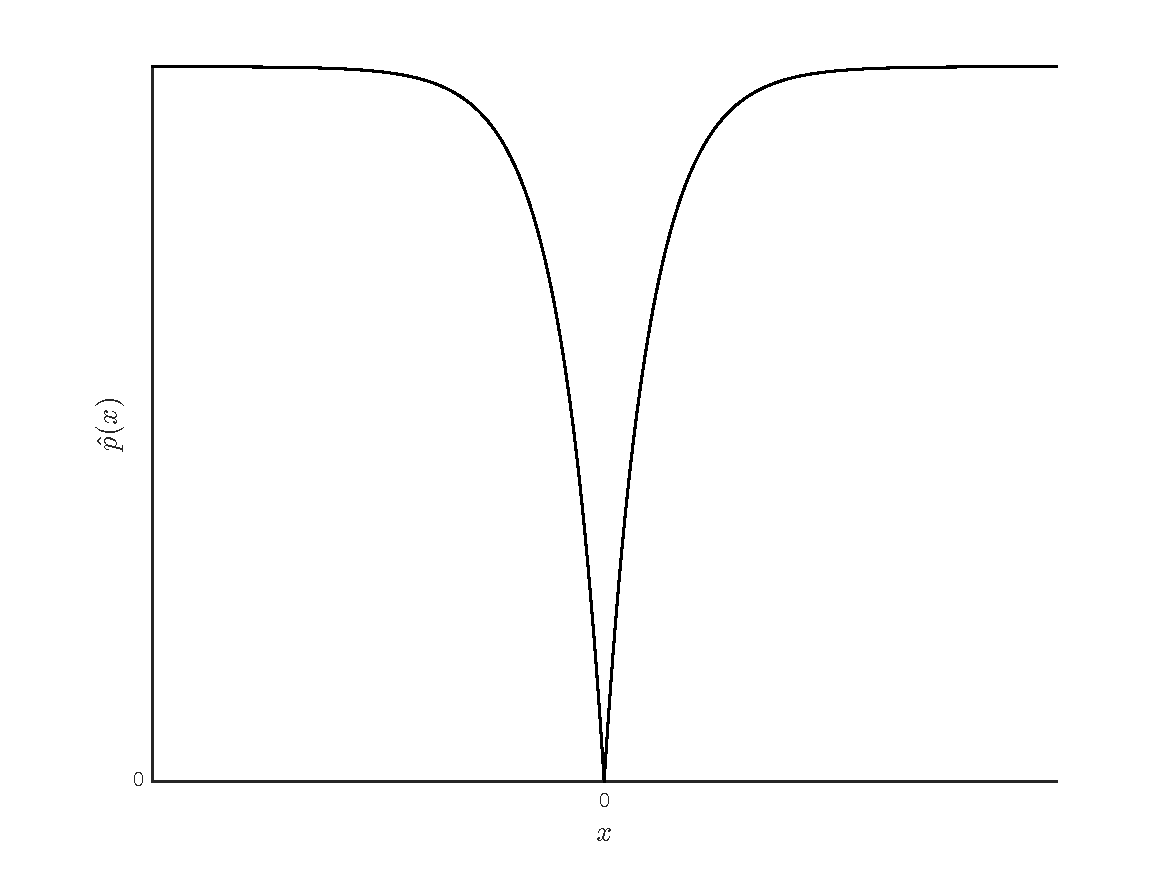
\includegraphics[width = 0.8\textwidth]{plot1.pdf}
			\end{figure}
			For $x \to \pm\infty$, the carrier concentration is not affected by the thin slice at $x = 0$.
			Therefore, the concentration is as if this slice does not exist.
			Therefore,
			\begin{align*}
				\lim\limits_{x \to \pm\infty} \hat{p}(x) & = G_{\text{optical}} \tau_p                                                                         \\
                                                                         & = \left( 10^{20} \si{\per\centi\metre\cubed\per\second} \right) \left( 10^{-5} \si{\second} \right) \\
                                                                         & = 10^{15} \si{\per\centi\metre\cubed}
			\end{align*}
		\item
			The carrier concentration profile $\hat{p}(x)$ for $x > 0$ is of the form
			\begin{align*}
				\hat{p}(x) & = A \left( 1 - e^{-\frac{x}{L_p}} \right)
			\end{align*}
			and for $x < 0$ is of the form
			\begin{align*}
				\hat{p}(x) & = A \left( 1 - e^{\frac{x}{L_p}} \right)
			\end{align*}
			Therefore, the concentration at $x \to \pm\infty$ can be approximated to the concentration at $x = \pm L_p$, where
			\begin{align*}
				L_p & = \sqrt{D_p \tau_p}                                                                                                                           \\
                                    & = \sqrt{\frac{k T}{q} \mu_p \tau_p}                                                                                                           \\
                                    & = \sqrt{\frac{k T}{q} \left( 350 \si{\centi\metre\squared\per\volt\per\second} \right) \left( 10^{-5} \si{\second} \right)}                   \\
                                    & = \sqrt{\left( 0.026 \si{\volt} \right) \left( 350 \si{\centi\metre\squared\per\volt\per\second} \right) \left( 10^{-5} \si{\second} \right)} \\
                                    & = \sqrt{91 \times 10^{-6} \si{\centi\metre\squared}}                                                                                          \\
                                    & = 9.54 \times 10^{-3} \si{\centi\metre}
			\end{align*}
	\end{enumerate}
\end{solution}

\begin{question}
	\begin{enumerate}
		\item
			Show that for a ladder of eigenvalues of $L_z$, for a given $l$,
			\begin{align*}
				\hat{L}^2 Y_{l m} & = \hbar^2 l (l + 1) Y_{l m}
			\end{align*}
			the lowest step in the ladder corresponds to
			\begin{align*}
				m_{\text{minimum}} & = -l
			\end{align*}
			Remember that
			\begin{align*}
				\hat{L}_z Y_{l m} & = \hbar m Y_{l m}
			\end{align*}
		\item
			We saw in recitation the following expression.
			\begin{align*}
				\hat{L}_- Y_{l m} & = B_{l m} Y_{l,m - 1}
			\end{align*}
			Find the coefficient $B_{l m}$ as a function of $l$ and $m$.
		\item
			Explain the following commutation relations, for the case of a central potential.
			You do not need to calculate anything.
			\begin{enumerate}
				\item $\left[ \hat{L}^2,\hat{H} \right] = 0$
				\item $\left[ \hat{L}_z,\hat{H} \right] = 0$
			\end{enumerate}
	\end{enumerate}
\end{question}

\begin{solution}
	\begin{enumerate}[leftmargin=*]
		\item
			For the lowest step in the ladder,
			\begin{align*}
				\hat{L}_- \hat{L}_z Y_{l m} & = 0
			\end{align*}
			Therefore,
			\begin{align*}
				\hat{L}_+ 0  & = \hat{L}_+ \hat{L}_- \hat{L}_z Y_{l m}                              \\
				\therefore 0 & = \hat{L}_+ \hat{L}_- Y_{l m}                                        \\
                                             & = \left( \hat{L}^2 - {\hat{L}_z}^2 + \hbar \hat{L}_z \right) Y_{l m} \\
                                             & = \left( \hbar^2 l (l + 1) - \hbar^2 m + \hbar^2 m \right) Y_{l m}
			\end{align*}
			Therefore,
			\begin{align*}
				l (l + 1)    & = m (m - 1) \\
				\therefore m & = -l
			\end{align*}
		\item
			\begin{align*}
				\hat{L}_- Y_{l m} & = B_{l m} Y_{l (m - 1)}
			\end{align*}
			Let
			\begin{align*}
				f & = \hat{L}_i Y_{l m} \\
				g & = Y_{l m}
			\end{align*}
			Therefore, the identity
			\begin{align*}
				\int\limits_{-\infty}^{\infty} f^*(x) \left( \hat{a}_{\pm} g(x) \right) \dif x & = \int\limits_{-\infty}^{\infty} \left( \hat{a}_{\mp} f(x) \right)^* g(x) \dif x
			\end{align*}
			implies
			\begin{align*}
                                & \quad \iint \left( \hat{L}_+ \hat{L}_- Y_{l m} \right)^* Y_{l m} \sin \theta \dif \theta \dif \varphi                         \\
                                & = \iint \left( \hbar^2 l (l + 1) - \hbar^2 m^2 + \hbar^2 m^2 \right) {Y_{l m}}^* Y_{l m} \sin \theta \dif \theta \dif \varphi \\
                                & = \hbar^2 \left( l (l + 1) - m (m - 1) \right)
			\end{align*}
			Also,
			\begin{align*}
				\iint \left( \hat{L}_- Y_{l m} \right)^* \left( \hat{L}_- Y_{l m} \right) \sin \theta \dif \theta \dif \varphi & = \left| B_{l m} \right|^2 \\
			\end{align*}
			Therefore,
			\begin{align*}
				\left| B_{l m} \right|^2 & = \hbar^2 \left( l (l + 1) - m (m - 1) \right) \\
				\therefore B_{l m}       & = h \sqrt{l (l + 1) - m (m - 1)}
			\end{align*}
		\item
			\begin{enumerate}[leftmargin=*]
				\item
					\begin{align*}
						\left[ \hat{L}^2,\hat{H} \right] & = 0
					\end{align*}
					As this commutation relation is zero, the two operators have common eigenfunctions.
				\item
					\begin{align*}
						\left[ \hat{L}_z,\hat{H} \right] & = 0
					\end{align*}
					As this commutation relation is zero, the two operators have common eigenfunctions.
			\end{enumerate}
	\end{enumerate}
\end{solution}

\begin{question}
	Consider a particle with the following wave function.
	\begin{align*}
		\Psi(r,\theta,\varphi) & = R(r) (2 Y_{0 0} + Y_{1 1} + 3 Y_{1 0} + 2 i Y_{1 (-1)})
	\end{align*}
	where $R(r)$ is a radial function and $Y_{l m}$ are the eigenfunctions of $\hat{L}^2$ and $\hat{L}_z$.
	\begin{enumerate}
		\item
			If $\hat{L}^2$ is measured for this state, what values can it have, and with what probabilities?
		\item
			Find the expectation value of $\hat{L}^2$ for this state.
		\item
			If $\hat{L}_z$ is measured for this state, what values can it have, and with what probabilities?
		\item
			Find the expectation value of $\hat{L}_z$ for this state.
	\end{enumerate}
\end{question}

\begin{solution}
	\begin{enumerate}[leftmargin=*]
		\item
			\begin{align*}
				\hat{L}^2 Y_{l m} & = l (l + 1) \hbar^2 Y_{l m}
			\end{align*}
			Therefore, the possible values of $L^2$ are the values of $l (l + 1) \hbar^2$ for $l = 0$ and $l = 1$.
			Therefore, the possible values of $L^2$ are $0$ and $2 \hbar^2$.\\
			~\\
			Let the constant of normalization for $\Psi$ be $A$.\\
			The probability corresponding to $Y_{0 0}$ is
			\begin{align*}
				\frac{|c_1|^2}{A} & = \frac{2^2}{A} \\
                                                  & = \frac{4}{A}
			\end{align*}
			The probability corresponding to $Y_{1 1}$ is
			\begin{align*}
				\frac{|c_2|^2}{A} & = \frac{1^2}{A} \\
                                                  & = \frac{1}{A}
			\end{align*}
			The probability corresponding to $Y_{1 0}$ is
			\begin{align*}
				\frac{|c_3|^2}{A} & = \frac{3^2}{A} \\
                                                  & = \frac{9}{A}
			\end{align*}
			The probability corresponding to $Y_{1 (-1)}$ is
			\begin{align*}
				\frac{|c_4|^2}{A} & = \frac{|2 i|^2}{A} \\
                                                  & = \frac{4}{A}
			\end{align*}
			Normalizing,
			\begin{align*}
				1            & = \sum c_k                \\
                                             & = \frac{4 + 1 + 9 + 4}{A} \\
                                             & = \frac{18}{A}            \\
				\therefore A & = 18
			\end{align*}
			Therefore,
			\begin{align*}
				P_1 & = \frac{2}{9}  \\
				P_2 & = \frac{1}{18} \\
				P_3 & = \frac{1}{2}  \\
				P_4 & = \frac{2}{9}
			\end{align*}
		\item
			\begin{align*}
				\left\langle L^2 \right\rangle & = \sum P_k {L^2}_k                                                                 \\
                                                               & = \frac{2}{9} 0 + \frac{1}{18} 2 \hbar + \frac{1}{2} 2 \hbar + \frac{2}{9} 2 \hbar \\
                                                               & = \frac{7}{9} 2 \hbar                                                              \\
                                                               & = \frac{14 \hbar}{9}
			\end{align*}
		\item
			\begin{align*}
				\hat{L}_z Y_{l m} & = m \hbar Y_{l m}
			\end{align*}
			Therefore, the possible values of $L_z$ are the values of $m \hbar$ for $m = 0$, $m = 1$, and $m = -1$.
			Therefore, the possible values of $L_z$ are $0$, $\hbar$, and $-\hbar$.\\
			~\\
			Let the constant of normalization for $\Psi$ be $A$.\\
			The probability corresponding to $Y_{0 0}$ is
			\begin{align*}
				\frac{|c_1|^2}{A} & = \frac{2^2}{A} \\
                                                  & = \frac{4}{A}
			\end{align*}
			The probability corresponding to $Y_{1 1}$ is
			\begin{align*}
				\frac{|c_2|^2}{A} & = \frac{1^2}{A} \\
                                                  & = \frac{1}{A}
			\end{align*}
			The probability corresponding to $Y_{1 0}$ is
			\begin{align*}
				\frac{|c_3|^2}{A} & = \frac{3^2}{A} \\
                                                  & = \frac{9}{A}
			\end{align*}
			The probability corresponding to $Y_{1 (-1)}$ is
			\begin{align*}
				\frac{|c_4|^2}{A} & = \frac{|2 i|^2}{A} \\
                                                  & = \frac{4}{A}
			\end{align*}
			Normalizing,
			\begin{align*}
				1            & = \sum c_k                \\
                                             & = \frac{4 + 1 + 9 + 4}{A} \\
                                             & = \frac{18}{A}            \\
				\therefore A & = 18
			\end{align*}
			Therefore,
			\begin{align*}
				P_1 & = \frac{2}{9}  \\
				P_2 & = \frac{1}{18} \\
				P_3 & = \frac{1}{2}  \\
				P_4 & = \frac{2}{9}
			\end{align*}
		\item
			\begin{align*}
				\left\langle L_z \right\rangle & = \sum P_k {L_z}_k                                                          \\
                                                               & = \frac{2}{9} 0 + \frac{1}{18} \hbar + \frac{1}{2} 0 + \frac{2}{9} (-\hbar) \\
                                                               & = \frac{\hbar}{18} - \frac{4 \hbar}{18}                                     \\
                                                               & = -\frac{3 \hbar}{18}
			\end{align*}
	\end{enumerate}
\end{solution}

\end{document}
